\section{Referencia de la Clase Pedido\-Proveedor\-View}
\label{classPedidoProveedorView}\index{PedidoProveedorView@{PedidoProveedorView}}
Muestra y administra la ventana con la informaci\'{o}n de un pedido a proveedor.  


{\tt \#include $<$pedidoproveedorview.h$>$}

Diagrama de herencias de Pedido\-Proveedor\-View\begin{figure}[H]
\begin{center}
\leavevmode
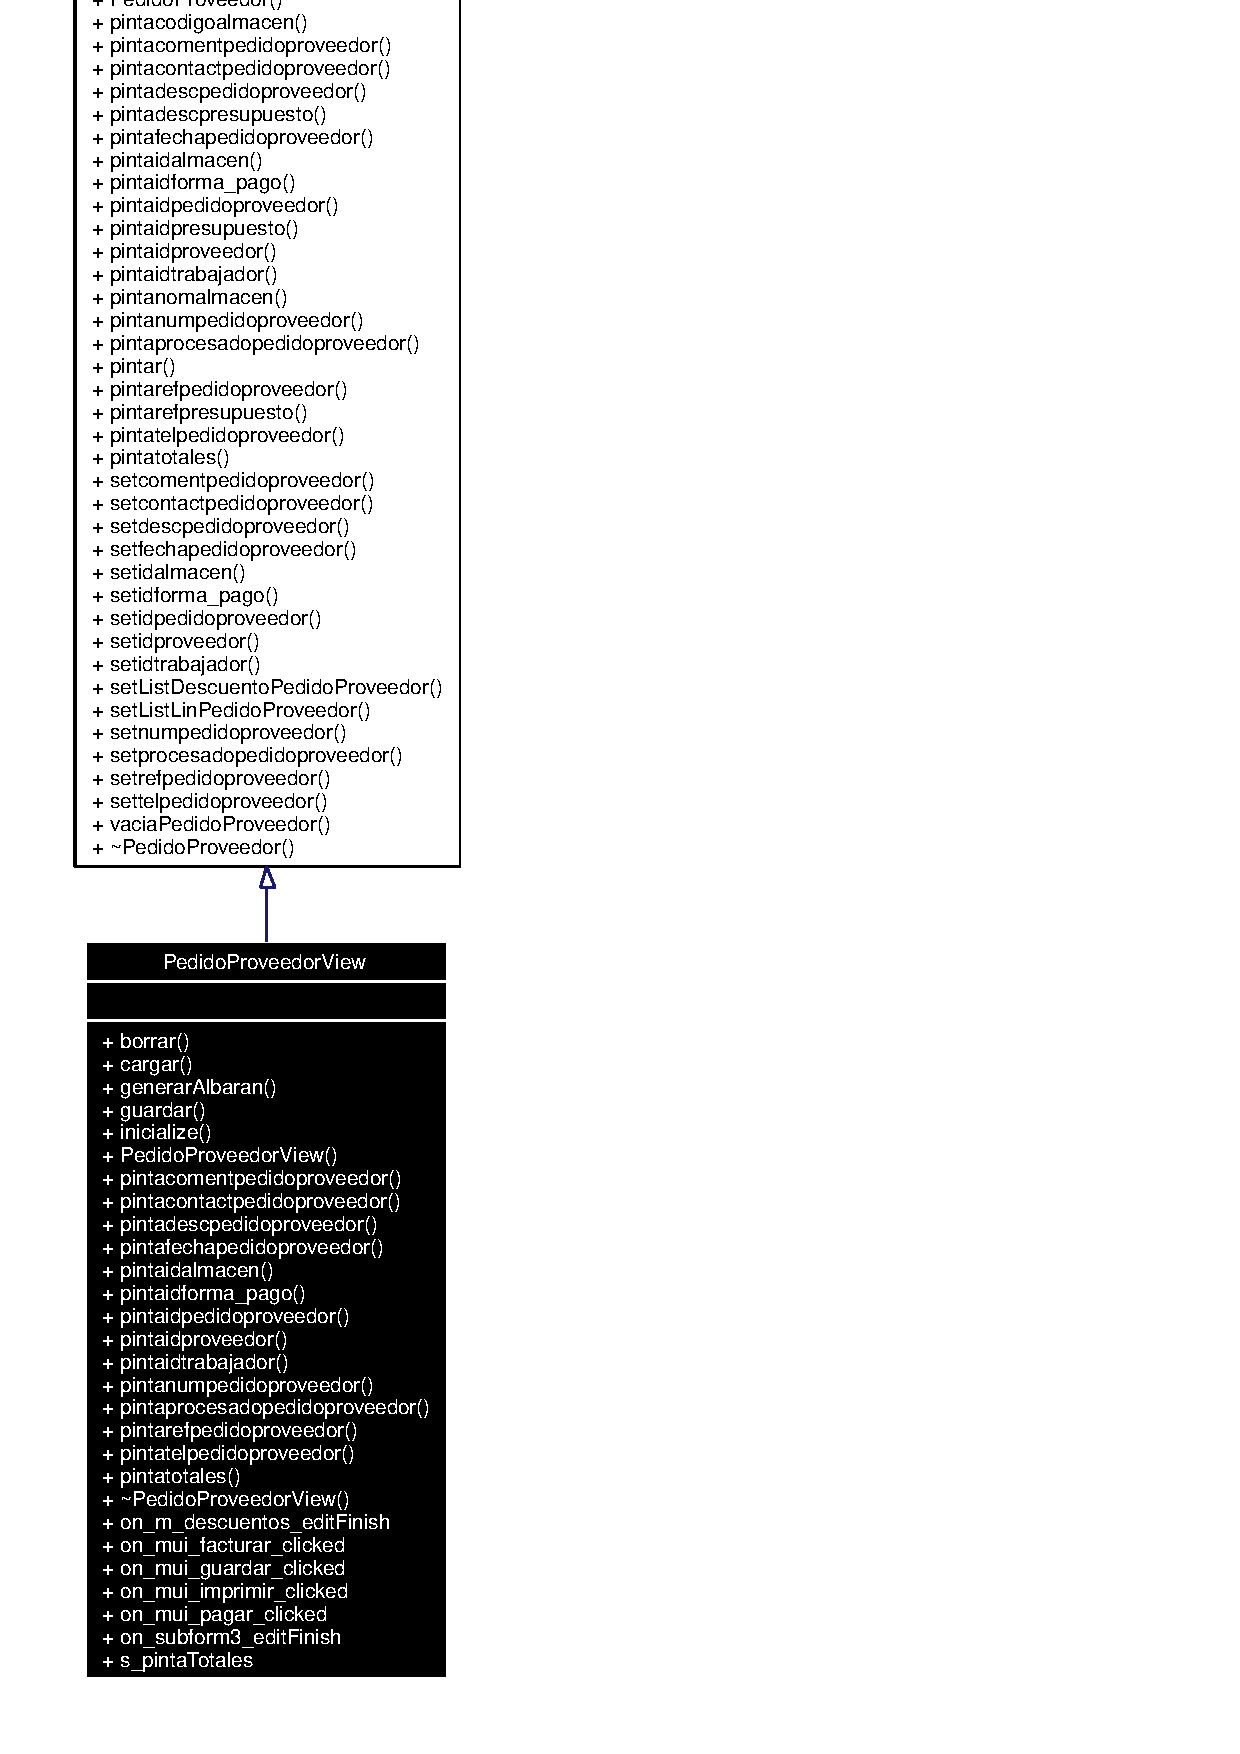
\includegraphics[width=110pt]{classPedidoProveedorView__inherit__graph}
\end{center}
\end{figure}
Diagrama de colaboraci\'{o}n para Pedido\-Proveedor\-View:\begin{figure}[H]
\begin{center}
\leavevmode
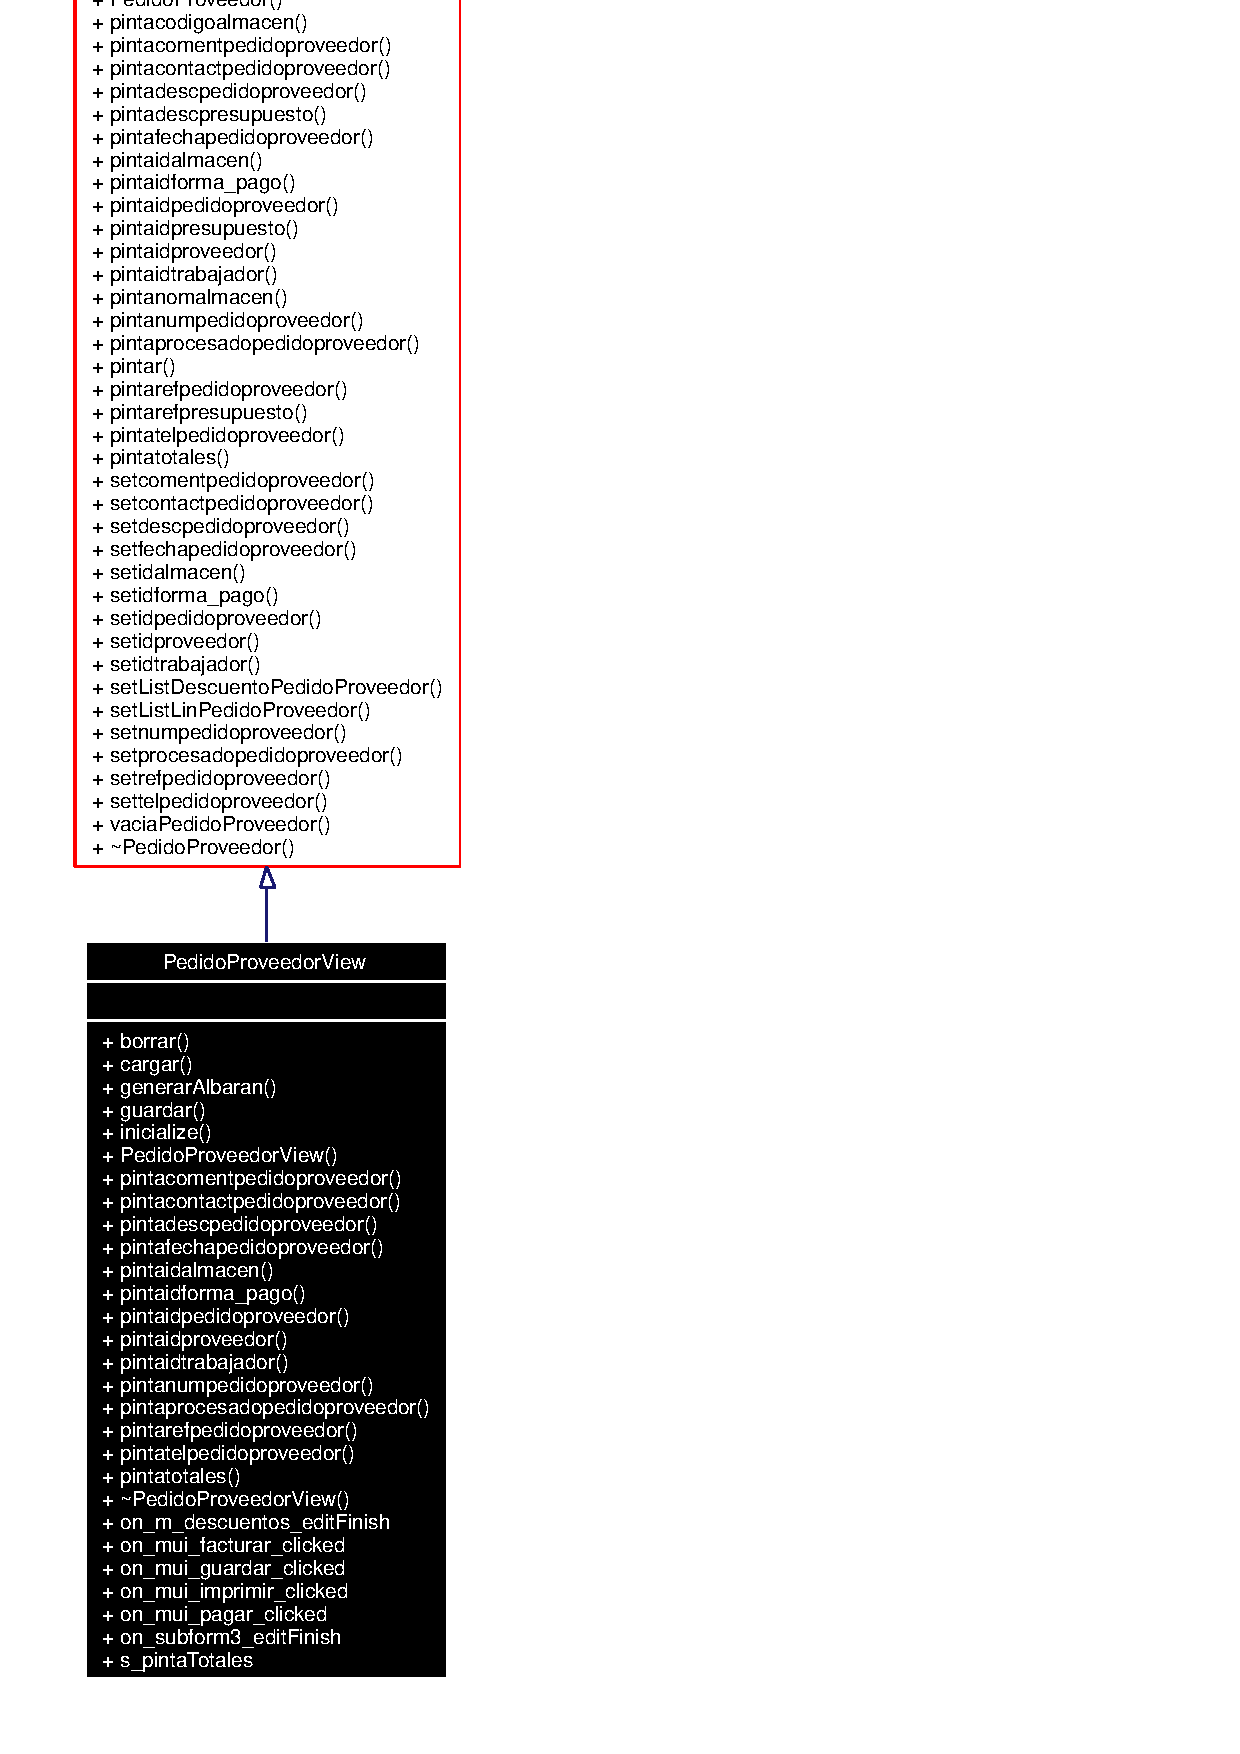
\includegraphics[width=110pt]{classPedidoProveedorView__coll__graph}
\end{center}
\end{figure}
\subsection*{Slots p\'{u}blicos}
\begin{CompactItemize}
\item 
virtual void {\bf on\_\-m\_\-descuentos\_\-edit\-Finish} (int, int)\label{classPedidoProveedorView_i0}

\item 
virtual void {\bf on\_\-mui\_\-facturar\_\-clicked} ()\label{classPedidoProveedorView_i1}

\item 
virtual void {\bf on\_\-mui\_\-guardar\_\-clicked} ()\label{classPedidoProveedorView_i2}

\item 
virtual void {\bf on\_\-mui\_\-imprimir\_\-clicked} ()\label{classPedidoProveedorView_i3}

\item 
virtual void {\bf on\_\-mui\_\-pagar\_\-clicked} ()\label{classPedidoProveedorView_i4}

\item 
virtual void {\bf on\_\-subform3\_\-edit\-Finish} (int, int)\label{classPedidoProveedorView_i5}

\item 
virtual void {\bf s\_\-pinta\-Totales} ()\label{classPedidoProveedorView_i6}

\begin{CompactList}\small\item\em Este slot se activa cuando hay cambios en los subformularios. \item\end{CompactList}\end{CompactItemize}
\subsection*{M\'{e}todos p\'{u}blicos}
\begin{CompactItemize}
\item 
virtual int {\bf borrar} ()\label{classPedidoProveedorView_a0}

\item 
virtual int {\bf cargar} (QString id)\label{classPedidoProveedorView_a1}

\begin{CompactList}\small\item\em Esta funcion carga un {\bf Pedido\-Proveedor}{\rm (p.\,\pageref{classPedidoProveedor})}. \item\end{CompactList}\item 
void {\bf generar\-Albaran} ()
\begin{CompactList}\small\item\em Se encarga de generar un albaran a partir del pedido. \item\end{CompactList}\item 
virtual int {\bf guardar} ()\label{classPedidoProveedorView_a3}

\begin{CompactList}\small\item\em Estos metodos deben existir para poder trabajar con la clase Ficha. \item\end{CompactList}\item 
void {\bf inicialize} ()
\item 
{\bf Pedido\-Proveedor\-View} ({\bf company} $\ast$, QWidget $\ast$parent=0)
\item 
void {\bf pintacomentpedidoproveedor} (QString id)\label{classPedidoProveedorView_a6}

\item 
void {\bf pintacontactpedidoproveedor} (QString id)\label{classPedidoProveedorView_a7}

\item 
void {\bf pintadescpedidoproveedor} (QString id)\label{classPedidoProveedorView_a8}

\item 
void {\bf pintafechapedidoproveedor} (QString id)\label{classPedidoProveedorView_a9}

\item 
void {\bf pintaidalmacen} (QString id)\label{classPedidoProveedorView_a10}

\item 
void {\bf pintaidforma\_\-pago} (QString id)\label{classPedidoProveedorView_a11}

\item 
void {\bf pintaidpedidoproveedor} (QString)\label{classPedidoProveedorView_a12}

\item 
void {\bf pintaidproveedor} (QString id)\label{classPedidoProveedorView_a13}

\item 
void {\bf pintaidtrabajador} (QString id)\label{classPedidoProveedorView_a14}

\item 
void {\bf pintanumpedidoproveedor} (QString id)\label{classPedidoProveedorView_a15}

\item 
void {\bf pintaprocesadopedidoproveedor} (QString id)\label{classPedidoProveedorView_a16}

\item 
void {\bf pintarefpedidoproveedor} (QString id)\label{classPedidoProveedorView_a17}

\item 
void {\bf pintatelpedidoproveedor} (QString id)\label{classPedidoProveedorView_a18}

\item 
void {\bf pintatotales} (Fixed iva, Fixed base, Fixed total, Fixed desc)\label{classPedidoProveedorView_a19}

\end{CompactItemize}


\subsection{Descripci\'{o}n detallada}
Muestra y administra la ventana con la informaci\'{o}n de un pedido a proveedor. 



\subsection{Documentaci\'{o}n del constructor y destructor}
\index{PedidoProveedorView@{Pedido\-Proveedor\-View}!PedidoProveedorView@{PedidoProveedorView}}
\index{PedidoProveedorView@{PedidoProveedorView}!PedidoProveedorView@{Pedido\-Proveedor\-View}}
\subsubsection{\setlength{\rightskip}{0pt plus 5cm}Pedido\-Proveedor\-View::Pedido\-Proveedor\-View ({\bf company} $\ast$ {\em comp}, QWidget $\ast$ {\em parent} = {\tt 0})}\label{classPedidoProveedorView_a5}


Usurpamos la identidad de mlist y ponemos nuestro propio widget con sus cosillas. 

\subsection{Documentaci\'{o}n de las funciones miembro}
\index{PedidoProveedorView@{Pedido\-Proveedor\-View}!generarAlbaran@{generarAlbaran}}
\index{generarAlbaran@{generarAlbaran}!PedidoProveedorView@{Pedido\-Proveedor\-View}}
\subsubsection{\setlength{\rightskip}{0pt plus 5cm}void Pedido\-Proveedor\-View::generar\-Albaran ()}\label{classPedidoProveedorView_a2}


Se encarga de generar un albaran a partir del pedido. 

Comprobamos que existe el elemento, y en caso afirmativo lo mostramos y salimos de la funcion.

Informamos de que no existe el pedido y a ver si lo queremos realizar. Si no salimos de la funcion.

Creamos el pedido. \index{PedidoProveedorView@{Pedido\-Proveedor\-View}!inicialize@{inicialize}}
\index{inicialize@{inicialize}!PedidoProveedorView@{Pedido\-Proveedor\-View}}
\subsubsection{\setlength{\rightskip}{0pt plus 5cm}void Pedido\-Proveedor\-View::inicialize ()}\label{classPedidoProveedorView_a4}


Inicializamos la forma de pago para que no se quede sin ser pintada. 

La documentaci\'{o}n para esta clase fu\'{e} generada a partir de los siguientes archivos:\begin{CompactItemize}
\item 
pedidoproveedorview.h\item 
pedidoproveedorview.cpp\end{CompactItemize}
